\chapter{Other static logics}
%------------------------------------------------------------------------%
\section{Pass-transistor}
This technology aim is to reduce the number of transistor with the idea to drive the mos by the gate and olso by the drain/source trerminal. It's a technology suited to implement adders and multipilers.\\
The main idea is to wathc the truth table of our function and think how to implement it as a multiplexer like in figure 

\centering
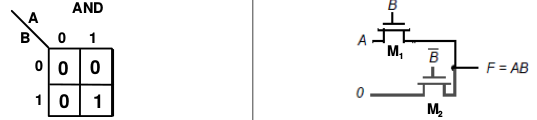
\includegraphics[width=0.35\textwidth]{C8_1.png}\\
\raggedright
 
The signal B is used as a selector.\\
This type of implementation has a lot of drawback since the nmos transistors are not good at charging capacitance they are affected by body effect so on the output node we have $V_{DD}-V_{tn}*$ that creates crossconduction current if it's connected to an inverter and it's the reason why it's forbidden to cascade pass-transistor.\\
%------------------------------------------------------------------------%
\subsection{Pass-transistor with level restorer}

First try to fix this issues is to use a level restorer in order to restore the voltage only to ground or power supply without consuming static power consumption using a classical inverter and a pmos 

\centering
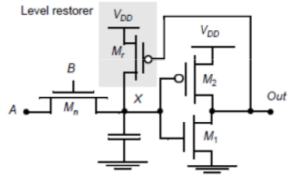
\includegraphics[width=0.35\textwidth]{C8_2.png}\\
\raggedright

The logic is still ratioed since the ratio of dimensions between the pass-transistor and the pmos it's foundamental since the pass-transistor have to be able to drive the X node low.\\
%------------------------------------------------------------------------%
\subsection{Swing restored pass transistor logic}

If we want a differential implementation of the pass-transistor logic we can employ two inverters in a crosscoupled fashon instead of the voltage restores and two complementary pass-transistor network.\\

\centering
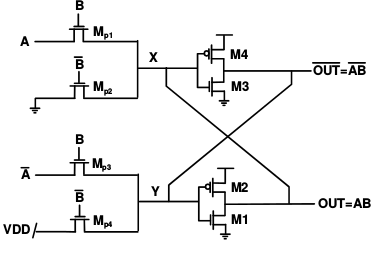
\includegraphics[width=0.35\textwidth]{C8_3.png}\\
\raggedright

The problem is again that this is still a ratioed implementation and a right sizing is mandatory to let this circuit work fine.\\




%------------------------------------------------------------------------%
%------------------------------------------------------------------------%
\section{Complementary pass-transistor logic CPL}
The final solution to the problems of the pass-transistor logic is the complementary pass transistor logic where we have two level restorers with gate connected to the opposite pass-transistor block and and two inverters that operates as buffer to permit the cascade of other logic ports.\\

\vspace{5mm}
\centering
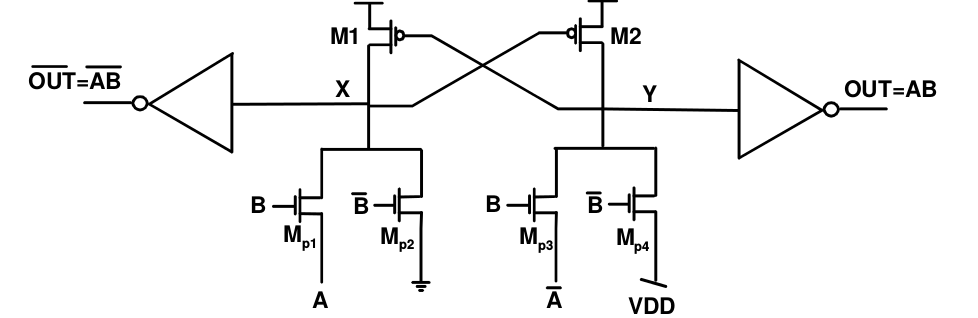
\includegraphics[width=0.5\textwidth]{C8_4.png}\\
\raggedright
\vspace{5mm}

This logic is ratioless since the feedback loop heps the transition and the on-off state of the two pmos transistors.\\
\vspace{5mm}
To build the pull down networks we have 2 different method: mux way or intuituve way.\\
In the multiplexer way we decide witch signals activate the mos and the signal that will be used as output than we can do some semplification limiting ourself to a tree structure like in figure

\vspace{5mm}
\centering
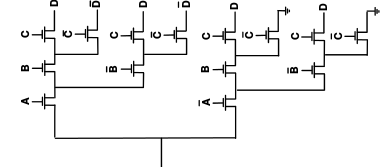
\includegraphics[width=0.5\textwidth]{C8_5.png}\\
\raggedright
\vspace{5mm}

The second way is to find on the k-map some groups of bits that corresponds to some condition like in figure

\vspace{5mm}
\centering
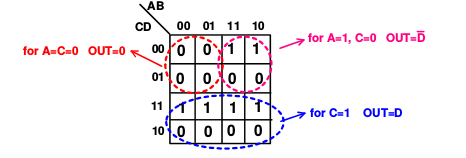
\includegraphics[width=0.5\textwidth]{C8_6.png}\\
\raggedright
\vspace{5mm}

\subsection{Propagation delay}
{\bf Low to high $\tau_{lh}$}\\
A low to high transition on the output Y corresponds to a high to low transition before the inverter so the nmos are discharging the intrinsic capacitance $C_{int}$.\\
The time taken by the system to discharge this capacitance is 
\begin{equation}
\tau'=\ln(2)R_nC_{int}
\end{equation}
where $R_n=13k$ as usual.\\
So the oveall time for a low to high transition is $\tau'$ plus the low to high propagation delay of the inverter that is 12ps
\begin{equation}
\tau_{lh}=\ln(2)R_nC_{int}+\tau_{plh}^{inv}=\ln(2)13kC_{int}+12ps
\end{equation}

\vspace{7mm}
{\bf High to low $\tau_{hl}$}\\
A high to low transition on the output Y corresponds to a low to high transition before the inverter so the nmos are charging the intrinsic capacitance $C_{int}$.\\
Thus we can't use the usual value of the resistance but we have to calculate the value considering an initial with source at 0V an final condition of the mos with source at $V_{DD}/2$.\\
\vspace{3mm}
\centering
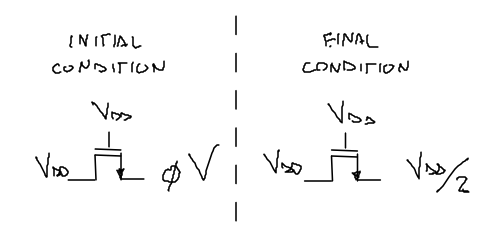
\includegraphics[width=0.55\textwidth]{C8_01.png}\\
\raggedright

Considering the body effect in the initial condition we are in velocity saturation but at the end in pinch off saturatio ($V_{tn}^{*}\simeq0.7-0.8$) so we can compute the equivalent resistance as 
\begin{equation}
R_{eq,n}=\frac{1}{2}\left(\frac{V_{DD}}{I_{vsat}^{(i)}}+\frac{V_{DD}/2}{I_{po}^{(f)}}\right)
\end{equation}
that depends on the equivalent reistance dimensions and it's the dominant term in the overall delay.\\
The high to low equivalent delay will be 
\begin{equation}
\tau_{hl}=\ln(2)R_{eq,n}C_{int}+\tau_{phl}^{inv}=\ln(2)R_{eq,n}C_{int}+18ps
\end{equation}

%------------------------------------------------------------------------%
\section{Trasmission gate}
Another solution to avoid the voltage drop problem is the use of trasmission gates that are one nmos and one pmos in parallel that are driven by complementary signals.\\
This device acts as a switch since turns on or off both devices. The advantage is that in this way we can always discharge/charge totally the load without stopping at a threshold voltage of distance.\\

\centering
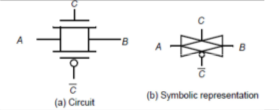
\includegraphics[width=0.35\textwidth]{C8_7.png}\\
\raggedright






























































